\documentclass[UTF8]{article}


\usepackage[zihao=-4]{ctex} % ctex可以写中文,中括号里那句的意思是正文小四号
\usepackage[a4paper]{geometry} % 调整纸张大小和页边距的包,这里中括号中规定了纸张大小
\usepackage{array}
\usepackage{fancyhdr}
\usepackage{amsmath}
\usepackage{multirow}
\geometry{left=2.5cm,right=2.5cm,top=2.5cm,bottom=2.5cm} % 页边距设置
\usepackage{caption}
\usepackage{graphicx} % 用它在报告里加图
\graphicspath{{figures/}} % 指定图片所在文件夹
\pagestyle{fancy}
\rhead{碰撞 }
\lhead{大学基础物理实验报告}
\cfoot{\thepage/7}
\rfoot{2023 年 3 月 10 日}

\begin{document}
	\thispagestyle{empty}
	\vspace*{0.5cm}
	
	\begin{figure}[h]
		\centering
		
\includegraphics[width=0.7\linewidth]{logo}
	\end{figure}
	\vspace*{0.1cm}
	\begin{center}
		\Huge{\textbf{大学基础物理实验报告}}\\
		\Huge{\textbf{《碰撞》}}
		
		\vspace*{0.1cm}
	\end{center}
	\begin{table}[h]
		\centering	
		\begin{Large}
			\begin{tabular}{p{3cm} p{5cm}<{\centering}}
				姓\qquad 名: & 蒋丰毅 \\
				\hline
				学\qquad 院: & 软件学院 \\
				\hline
				学\qquad 号: & 2211082 \\
				\hline
				分\qquad 组: & C组10号 \\
				\hline
				实验时间: & 2023.3.9\\
				\hline
				指导教师: & 董晋阳\\
				\hline
			\end{tabular}
		\end{Large}
	\end{table}
	\clearpage
	\normalsize
	\begin{center}
		\LARGE\textbf{碰撞}
	\end{center}
	\subsection*{[实验目的要求]}
	\par 1.用对心碰撞特例检验动量守恒定律。
	\par 2.了解动量守恒和能量守恒的条件。
	\par 3.熟练的使用气垫导轨及数字毫秒计。

	
	\subsection*{[实验仪器用具]}
	\par 气垫导轨(包括滑块和挡光框一对);数字毫秒计;物理天平及游标卡尺
	\subsection*{[实验原理简述]}
	\subsubsection*{动量守恒定理}
	\par 动量守恒定理指出:若一个物体系所受合外力为零,则物体的总动量保持不变;若物体系所受合外力在某个方向的分量为零。则此物体系的总动量在该方向上的分量守恒。本实验在平直导轨上,两个滑块作对心碰撞。忽略空气阻力,则在水平方向上满足没有外力的条件,即满足动量守恒定律。
	\begin{equation}
		m_1u_1+m_2u_2=m_1v_1+m_2v_2
	\end{equation}
	\par 分别测出$(1)$式中各量,若等式两边相等,则动量守恒定律得到验证。
	\subsubsection*{碰撞后的动能损失}
	\par 碰撞过程中的动能是否守恒,与碰撞的性质有关,用恢复系数$e$来表达:
	\begin{equation}
		e=\frac{v_2-v_1}{u_1-u_2}
	\end{equation}
	\par 在$(2)$式中,分母和分子分别为碰撞前后两者的相对速度。
	\par (1)完全弹性碰撞:若相互碰撞的物体材料为弹性材料,碰撞后形变完全恢复,则物体的总动能不变,此时$e=1$,没有能量损失。
	\par (2)非弹性碰撞:若相互碰撞的物体材料有一定弹性,碰撞后有部分形变残留,则物体的总动能有所损耗,此时$0\textless e\textless1$,有部分能量损失。
	\par (3)完全非弹性碰撞:若相互碰撞的物体完全没有弹性,在碰撞之后粘在一起继续运动,此时$v_1=v_2$,故$e=0$,物体系的能量损失达到最大。
	\subsubsection*{实验的假设和误差分析}
	\par 本实验使用的物体质量$m_1=m_2\equiv m$且$u_2=0$,当发生的是完全弹性碰撞是(本实验通过使用弹簧来模拟这一点),式(1)和式(2)的解为:
	\begin{equation}
		\left\{
		\begin{matrix}
			v_1=0 \\
			v_2=u_1 \\
		\end{matrix}
		\right.
	\end{equation}
	\par 这表明,当两块滑块质量相等,且第二块滑块处于静止时发生完全弹性碰撞,第二块滑块会“继承”第一块滑块的速度,“接力式”地向前运动。只需(3)式子得到验证,则说明完全弹性碰撞中动量守恒,动能也守恒。
	\par 以上时理想化的模型。若两块滑块的质量不严格相等,两挡光物的有效遮光宽度$\Delta s_1$和$\Delta s_2$也不严格相等,则碰撞后的动量百分差为$E_1$为
	\begin{equation}
		E_1=\frac{\vert p_2-p_1 \vert}{p_1}=\vert \frac{m_2\Delta s_2\Delta t_1}{m_1\Delta s_1\Delta t_2}-1 \vert
	\end{equation}
	\par 动能的百分差$E_2$为
	\begin{equation}
		E_2=\frac{\vert E_{k2}-E_{k1} \vert}{E_{k1}}=\vert \frac{m_2\Delta s_2^2\Delta t_1^2}{m_1\Delta s_1^2\Delta t_2^2}-1 \vert
	\end{equation}
	\par 若$E_1$和$E_2$都在误差范围之内,则说明上述结论成立。
	\vspace*{1cm}
	\par 对于完全非弹性碰撞,式(1)和式(2)的解为
	\begin{equation}
		v_1=v_2\equiv v=\frac{u_1}{2}
	\end{equation}
	\par 若(6)式得证,则说明完全非弹性碰撞动量守恒,且$e=0$,其动能损失最大,约为$50\%$.
	\par 考虑到两次速度测量使用的都是第一块滑块的挡光物,故$\Delta s_1^{'} \equiv \Delta s_2^{'}$,同样求得动量和动能百分差$E_1^{'}$和$E_2^{'}$分别为
	\begin{equation}
		E_1^{'}=\frac{\vert p_2^{'}-p_1^{'} \vert}{p_1^{'}} =\left\vert \left(1+\frac{m_2}{m_1}\right)\frac{\Delta t_1^{'}}{\Delta t_2^{'}}-1 \right\vert
	\end{equation}
	\begin{equation}
			E_2^{'}=\frac{\vert E_{k2}^{'}-E_{k1}^{'} \vert}{E_{k1}^{'}}=\left\vert \left(1+\frac{m_2}{m_1}\right)\left(\frac{\Delta t_1^{'}}{\Delta t_2^{'}}\right)^2-1 \right\vert
	\end{equation}
	 其动能损失的百分误差为
	 \begin{equation}
	 	E_{\Delta} = \left\vert 2\left(1+\frac{m_2}{m_1}\right)\left(\frac{\Delta t_1^{'}}{\Delta t_2^{'}}\right)^2-1 \right\vert
	 \end{equation}

	 \clearpage
	 \par 若$E_1^{'}$和$E_{\Delta}$都在其实验误差范围之内,则说明上述结论成立。
	 \subsection*{[实验步骤]}

  	\subsubsection*{动态调零和调重}
  	\par 取两个滑块分别放在电子天平上,测得两滑块的质量分别为$m_1=131.58g$,$m_2=131.51g$,误差$\Delta m = 0.07g<0.1g$。打开气泵和数字毫秒计,等待一段时间后将滑块1放在导轨上并给予初速度,观察数字毫秒计上显示的滑块通过两次光电门的时间,若两次的时间差大于$0.1ms$,则保持旋钮$Q$不动,调节旋钮$P$,重复试验直到两者差值小于$0.1ms$为止。本次试验动态调平时时间分别为$54.15ms$,$54.24ms$。
  		\begin{figure}[h]
  		\centering
  		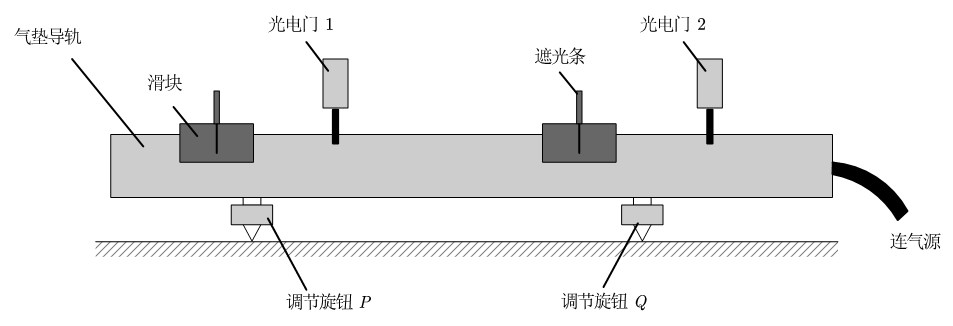
\includegraphics[width=1\linewidth]{气垫导轨}
  		\caption{气垫导轨示意图} %caption是图片的标题
  	\end{figure}
  	\subsubsection*{动量定理的验证}
  	\par 调节两个滑块的方向,使得滑块上的弹簧同时向内,同时调节遮光条的方向使得其能被光电门检测到。将两个滑块和光电门按照图1的位置关系摆放。用手保持右边的滑块不动,给予左侧的滑块初速度,记录下左侧滑块第一次通过左侧光电门和碰撞后右边滑块第一次通过右边光电门的时间,重复三次,结果记录在数据处理中。
  	\subsubsection*{动能损失量的测定}
  	\par 和动量定理步骤大致一样,不同点在于将两个滑块调换位置,使得两滑块尾部的魔术贴向内,碰撞后两个滑块会一起运动,且记录的是左侧滑块两次通过光电门的时间(即数字毫秒计第一次和第三次的记录),重复三次,结果记录在数据处理中。
  	\subsubsection*{$\Delta s$的测量}
  
  	\par 本实验中采用了$S_2$计时法:测量光电门两次挡光的间隔时间。故测量值应为图2中标注的$\Delta s$,由于不方便直接测量,使用了$\Delta s=\Delta L -\Delta d$间接测量。由于是同样的一块滑块,故第二次测量只测量了一次。最后根据公式$v=\frac{\Delta s}{\Delta t}$求出速度并计算恢复系数$e$,动量百分差$E_1$及能量百分差$E_2$.
  		\begin{figure}[h]
  		\centering
  		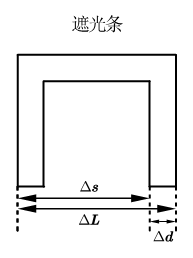
\includegraphics[width=0.3\linewidth]{遮光条}
  		\caption{遮光条示意图} %caption是图片的标题
  	\end{figure}
  \subsection*{[数据处理]}
\[\Delta s_1=0.04996m \quad \Delta s_2=0.04996m \quad \Delta s_1^{'}=0.04996m \]
	\par 根据$v = \dfrac{s}{t}$可得

	\begin{table}[h]
		\centering
		\begin{tabular}{|l|llll|llll|}
			\hline
			\multirow{3}{*}{次数i} & \multicolumn{4}{l|}{完全弹性碰撞}                                                            & \multicolumn{4}{l|}{完全非弹性碰撞}                                                           \\ \cline{2-9} 
			& \multicolumn{2}{l|}{碰前}                              & \multicolumn{2}{l|}{碰后}         & \multicolumn{2}{l|}{碰前}                              & \multicolumn{2}{l|}{碰后}         \\ \cline{2-9} 
			& \multicolumn{1}{l|}{$\Delta t_1/s$}     & \multicolumn{1}{l|}{$u/(m\cdot s^{-1})$} & \multicolumn{1}{l|}{$\Delta t_2$}     & $v$ & \multicolumn{1}{l|}{$\Delta t_1^{'}$}     & \multicolumn{1}{l|}{$u^{'}$} & \multicolumn{1}{l|}{$\Delta t_2^{'}$}     & $u^{'}$ \\ \hline
			1                    & \multicolumn{1}{l|}{0.06359} & \multicolumn{1}{l|}{0.78565} & \multicolumn{1}{l|}{0.06366} & 0.78479 & \multicolumn{1}{l|}{0.07552} & \multicolumn{1}{l|}{0.66154} & \multicolumn{1}{l|}{0.14939} & 0.33442 \\ \hline
			2                    & \multicolumn{1}{l|}{0.05673} & \multicolumn{1}{l|}{0.88066} & \multicolumn{1}{l|}{0.05863} & 0.85212 & \multicolumn{1}{l|}{0.04943} & \multicolumn{1}{l|}{1.01072} & \multicolumn{1}{l|}{0.09996} & 0.49979 \\ \hline
			3                    & \multicolumn{1}{l|}{0.08242} & \multicolumn{1}{l|}{0.60616} & \multicolumn{1}{l|}{0.08289} & 0.60272 & \multicolumn{1}{l|}{0.05596} & \multicolumn{1}{l|}{0.89278} & \multicolumn{1}{l|}{0.11162} & 0.44759 \\ \hline
		\end{tabular}
		\caption{时间记录及速度计算}
	\end{table}
	\subsubsection*{恢复系数e的计算}
	对于完全弹性碰撞,根据公式$e=\dfrac{v_2-v_1}{u_1-u_2}$易得
	\[e_1 = \frac{0.78479}{0.78565}=0.998900 \]
	\[e_2 = \frac{0.85212}{0.88066}=0.967593\]
	 \[e_3 = \frac{0.60272}{0.60616}=0.994329\]
	 \par 对于完全非弹性碰撞,由于两个滑块一起运动,故$e=0$
	 \subsubsection*{动量和动能百分差}
  	\par 对于完全弹性碰撞,根据公式(4)(5)计算可得
  	\[E_{11}=0.01631\quad E_{12} = 0.03292\quad E_{13} = 0.00619\]
  	\[E_{21}=0.00272\quad E_{22}=0.06426 \quad E_{23}=0.01183\]
  	\par 对于完全非弹性碰撞,根据公式(7)(8)计算可得
  	\[E_{11}^{'}=0.01077 \quad E_{12}^{'}=0.01126 \quad E_{13}^{'}=0.00242\]
  	\[E_{21}^{'}=0.02193 \quad E_{22}^{'}=0.02214 \quad E_{13}^{'}=0.00511\]
  	\subsection*{[误差分析]}
  	\par 从动能和动量百分差的关系来看,实验中速度越快的组别,误差越大。从动态调平的过程来看,由于存在着空气阻力,导致动态调平后导轨并不是真正的水平,而是存在着一个倾角。动态调平和静态调平无法同时满足。这也解释了为什么实验过程中要用手扶住静止的小车。正是由于这个倾角的存在,沿着导轨向下的重力分量与空气阻力相互抵消,但根据
  	\[f=kx\]
  	\par 这样的相互抵消只在调平时的速度情况下满足,而对于其他的速度,由于速度的改变,速度越快的组别空气阻力的影响越大,导致实验结果误差也越大。
  	\par
  	\par 另外,本实验还出现了这样的状况:两个滑块的弹簧缠绕在一起。这是由于两个滑块不是对心碰撞产生的,由此可见,即使是调整之后,也不一定能保证两个滑块的质心同时处在运动路径的直线上,最终导致了实验误差。
  	\subsection*{[思考题]}
  	\par 1.完全弹性碰撞后,物体的形变完全恢复,恢复系数为1,且动能没有损失。
  	\begin{align*}
		\begin{cases}
  			m_1u_1+m_2u_2=m_1v_1+m_2v_2 \\
  			\dfrac{1}{2}m_1u_1^2+\dfrac{1}{2}m_2u_2^2=\dfrac{1}{2}m_1v_1^2+\dfrac{1}{2}m_2v_2^2 \\
  		\end{cases}
  	\end{align*}
  	\par 变形为
  	\begin{align*}
  		\begin{cases}
  			m_1(u_1-v_1)=m_2(v_2-u_2)\\
  			m_1(u_1-v_1)(u_1+v_1)=m_1(v_2-u_1)(v_2+u_1)
  			 \\
  		\end{cases}
  	\end{align*}
  \par 相除即得
  \[v_2-v_1=u_2-u_1\]
  \par 2.由于$m>>m_1$由动量定理,导轨的速度变化量可以忽略不计,故
  \[e=\frac{v-0}{v-0}=1\]
  \par 3.因为本实验应做到尽量只考虑水平方向上的动量,若不是对心碰撞,会产生竖直方向上的误差。在本次实验中,通过观察和确定滑块上的弹簧圈牢固且没有变形来尽量保证这一点。
  \par 4.由对称性可知,若发生完全非弹性碰撞,则两个滑块将会停在原地,若发生弹性碰撞,则两个滑块将以大小相同方向相反的速度分离。
  \par 5.尽量使实验速度靠近调平速度;尽量使滑块对心碰撞;实验前一定要保证两滑块质量相等;保证滑块运动稳定不摇晃。
  	

\end{document}